\documentclass{ceurart}

\usepackage{listings}
\lstset{breaklines=true}

\usepackage{xspace}
\usepackage{xcolor}
\usepackage{relsize}
\usepackage{tikz}
\usepackage{tabularx}
\usepackage{multirow}
\usepackage{sourcecodepro}

\usetikzlibrary{arrows.meta}
\usetikzlibrary{positioning}

\newcommand{\todo}[1]{\textcolor{blue}{#1}}
\newcommand{\todocite}{\todo{[CITE]}\xspace}

\newcommand{\Ni}{(1)~}
\newcommand{\Nii}{(2)~}
\newcommand{\Niii}{(3)~}
\newcommand{\Niv}{(4)~}
\newcommand{\Nv}{(5)~}
\newcommand{\Na}{(a)~}
\newcommand{\Nb}{(b)~}
\newcommand{\Nc}{(c)~}
\newcommand{\Nd}{(d)~}
\newcommand{\Ne}{(e)~}

\newcommand{\textttsmall}[1]{\texttt{\smaller #1}}
\newcommand{\query}[1]{\textttsmall{#1}}
\newcommand{\Bert}{\textsc{Bert}\xspace}
\newcommand{\iraxioms}{\textttsmall{ir\_axioms}\xspace}
\newcommand{\nDCG}[1]{nDCG\def\tempndcg{#1}\ifx\tempndcg\empty\else{@}\tempndcg\fi}
\newcommand{\map}{MAP}
\newcommand{\KwikSort}{\textsc{KwikSort}\xspace}

\begin{document}

\copyrightyear{2022}
\copyrightclause{%
  Copyright for this paper by its authors.
	Use permitted under Creative Commons License Attribution~4.0
	International~(CC~BY~4.0).%
}
\conference{%
  CLEF~2021 -- 
  Conference and Labs of the Evaluation Forum, 
	September~5--8,~2022,
  Bologna, Italy%
}

\title{%
  Grimjack at \texorpdfstring{Touché~2022}{Touché 2022}:\texorpdfstring{\\}{ }
  Axiomatic Reranking and Query Reformulation%
}
\title[mode=sub]{%
  Notebook for the Touché Lab on Argument Retrieval at CLEF\ 2022%
}

\author{Jan Heinrich Reimer}[
  orcid=0000-0003-1992-8696,
  email=jan.reimer@student.uni-halle.de,
  url=https://heinrich.reimer.family,
]
\author{Johannes Huck}[
  email=johannes.huck@student.uni-halle.de,
  url=https://github.com/johannes-huck,
]
\author{Alexander Bondarenko}[
  orcid=0000-0002-1678-0094,
  email=alexander.bondarenko@informatik.uni-halle.de,
  url=https://alexanderbondarenko.com/,
]

\address{%
  Martin-Luther-Universität Halle-Wittenberg,
  06099~Halle~(Saale), Germany
}

\begin{abstract}
  We, Team Grimjack, present \todo{four} approaches for answering comparative questions, submitted to the Touché Lab on Argument Retrieval.
  Our approaches follow two objectives: ranking argumentative and high-quality documents first, and exposing arguments of different stances towards the compared objects fairly in high ranking positions.
  We therefore propose a multi-stage retrieval pipeline with query reformulation and merging, baseline retrieval, quality and stance tagging, and different task-specific re-ranking steps.
  First, we re-rank aiomatically based on argumentative retrieval axioms.
  Second, we re-rank to ensure fair exposure across argument stances.
  In all retrieval steps, we use the T0 language model to evaluate whether zero-shot language models can successfully answer comparative questions.
\end{abstract}

\begin{keywords}
  Axiomatic Reranking \sep
  Query Reformulation \sep
  T0 \sep
  Argument Quality \sep
  Argument Stance \sep
  CEUR-WS
\end{keywords}


\maketitle

\section{Introduction}\label{intro}

%Current information retrieval systems are well able to answer keyword queries or simple questions but answering comparative questions is still a challenging task~\cite{BondarenkoGFBAPBSWPH2021}.
Argument retrieval is a specific task that not only considers topical relevance of retrieved documents to given queries (usually of controversial, argumentative or opinion nature) but also accounts for argument specific features like argument quality and stance~\cite{BondarenkoFBGAPBSWPH2020, BondarenkoGFBAPBSWPH2021}.  
Furthermore, it has been shown that current search engines might return biased results~\cite{ShahB2022} and argument retrieval systems return ``unfairelly'' distributed pro / con arguments~\cite{CherumanalSSC2021}. We especially emphasize the importance of retrieving diverse results for comparative questions (e.g., ``Train or plane? Which is the better choice?'') that provide different point of views to mitigate biasing users' decisions towards one or the other comparison option.

%\citet{BondarenkoFKSGBPBSWPH2022} organize the Touché Lab on Argument Retrieval at CLEF to find different promising approaches that tackle the task of retrieving arguments to comparative questions from a web-scale collection of passages.
%The retrieved arguments should be of high rhetorical an argumentative quality but also relevant to the query.
%Additionally, in~2022 the participants of the Touché shared task should also tag their resulting passages with their stance towards the comparative objects.
%Answering comparative questions supports users in their everyday lives but users might struggle with converting those natural language questions into keyword queries~\cite{BondarenkoGFBAPBSWPH2021}.

Our Team Grimjack participated in the Touch{\'e} shared task on Argument Retrieval for Comparative Questions which goals are: \Ni To retrieve relevant and high quality argumentative passages from a collection of 0.9~million text passages to a set of 50~search topics and \Nii to classify the stance of the retrieved passages towards the comparison objects in search topics~\cite{BondarenkoFKSGBPBSWPH2022}. As part of our participation in the task, we have developed a flexible retrieval pipeline in Python based on Pyserini~\cite{LinMLYPN2021} as an easily configurable command line application. In the first step, our approach uses query (comparative questions from topics' titles) reformulation and expansion by important terms from topics descriptions and narratives. Then the top~\todo{X} initially retrieved passages using query likelihood with Dirichlet smoothing~\todocite are axiomatically re-ranked based on the \todo{number} of premises and claims \todo{identified with} and argument quality predictions by the \todo{classifier}. Finally, the pro and con argumentative passages towards the comparative objects are balanced in the final ranking by \todo{method} (cf.\ Section~\ref{approach} for more details on the approach and submitted runs).

Additionally, we manually labeled the \todo{relevance} of \todo{XX} documents for three topics returned by our system (before the official results are made available by the organizers). Our manual assessment shows the potential of expanding queries with synonyms and contextual information for improving the effectiveness of our argument retrieval approach~(cf.\ Section~\ref{evaluation}).

%We develop a flexible retrieval pipeline to participate in the Touché shared task on argument retrieval for comparative questions~(c.f. Section~\ref{approach}).
%Our approach is developed with Python and Pyserini~\cite{LinMLYPN2021} as an easily configurable command line application.
%With query reformulation, expansion and combination we relax the initial query and exploit additional topic context such as description and narrative.
%After retrieving candidate passages using query likelihood with Dirichlet smoothing, we tag each passage's argumentative structure, argument quality and the stance towards the comparative objects.
%To improve relevance and quality on high ranks, we then re-rank results axiomatically using specialized argumentative retrieval axioms, incorporating the previously annotated argument quality.

%Two strategies to balance the passages' stances towards the comparative objects showcase fair re-ranking for arguments.

%Even though we were unable to transfer enough relevance judgements from previous editions of the Touché shared tasks, our manual assessment of three topics shows the potential of expanding queries with synonyms and contextual information~(c.f. Section~\ref{evaluation}).

%% The last statement could fit in the CR version depending on the final evaluation: good or bad
%Different configurations for our submitted runs should pose examples to discuss current doubts about the usefulness of large zero-shot language models like T0++~\cite{SanhWRBSACSLRDBXTSSKCNDCJWMSYPBWNRSSFFTBGBWR2021} in the field of argumentative information retrieval~\cite{ShahB2022}.

\section{Related Work}
    Since the shared task, we participated in is in its third edition this year the most related work has been done in the two previous years. So we will have a look at the years 2020 and 2021 of the Touché shared task 2: Answering of Comparative Questions.
    \subsection{Touchè 2020: Argument Retrieval}
        In 2020 the task was to retrieve documents from the ClueWeb12 corpus to answer comparative questions like \textit{Is X better than Y with respect to Z?}. The resulting documents should contain documents with convincing arguments for or against the comparative questions in contrast to current search engines which may display only one (short) answer. For this task, five teams submitted eleven runs. We now will have a look at the two best runs: Team Bilbo Baggins and Team Inigo Montoya~\cite{BondarenkoFBGAPBSWPH2020}\par
        Team Bilbo Baggins has developed a retrieval pipeline with four steps. In their first one, they analyze the query and determine entities that compare. Then they expand the queries with synonyms and antonyms of the found entities and send those queries to ChatNoir\footnote{\url{https://www.chatnoir.eu/}}. In the second step, they conduct argument mining and calculate the document quality by evidence mining and link analysis. The third step consists of summing up the collected scores and building relevance, support, and credibility scores. In their final step, they build weighting scores and rerank the documents by multiplying the weighting scores with the sum of the aforementioned scores. Team Bilbo Baggins scored first place in 2020 with an NDCG@5 score of 0.580~\cite{AbyeST2020}.\par
        The second place in 2020 (Team Inigo Montoya) queries ChatNoir with the original queries and processes the first 20 results further. These results are sent to TARGER~\cite{ChernodubOHBHBP2019} to determine their premise and claims. Arguments from one web page will then be stored in one document. These argument documents will then be indexed and queried with Okapi BM25 and the top 20 results will be displayed. Team Inigo Montoya scored a NDCG@5 of 0.567~\cite{Huck2020}.
    \subsection{Touchè 2021: Argument Retrieval}
        The task for 2021 was the same as for 2020. So participants were asked to retrieve relevant documents from the ClueWeb12 corpus for comparative questions. However, the provided topics and therefore the queries have been changed. In 2021 there were six submitted runs. We now will have a look at the two best runs regarding the NDCG@5: Team Katana and Team Thor~\cite{BondarenkoFBGAPBSWPH2021}\par
        Team Katana queries the search engine ChatNoir with the provided topics and extracts up to 100 unique documents from the result set. Then they clean the documents. After that, they rerank the documents by one of their developed models. Their models are feature-based machine learning models with features from PyTerrier, specific comparative features, and scores from the ChatNoir system. They developed the following ranking models: (1) an XGBoost approach, (2) a LightGBM approach, (3) Random Forests, and (4) a BERT-based
        ranker. Team Katana scored first place with an NDCG@5 of 0.489~\cite{ChekalinaP2021}.\par
        Team Thor queries the search engine ChatNoir with an AND-Operator and removes every punctation from the topics and the documents found. Additionally, they remove all boilerplate from the documents to extract the main content. Then they create an index with Elasticsearch of the first 110 documents returned by ChatNoir. After that, they expand the original query with synonyms from WordNet. Here for every word synonyms will be calculated. Lastly, they query their index with Okapi BM25 (b=0.68 and k1=1.2). Team Thor achieved an NDCG@5 of 0.478~\cite{ShirshakovaW2021}. 


\section{Approach}\label{approach}

\begin{figure}
	\centering
    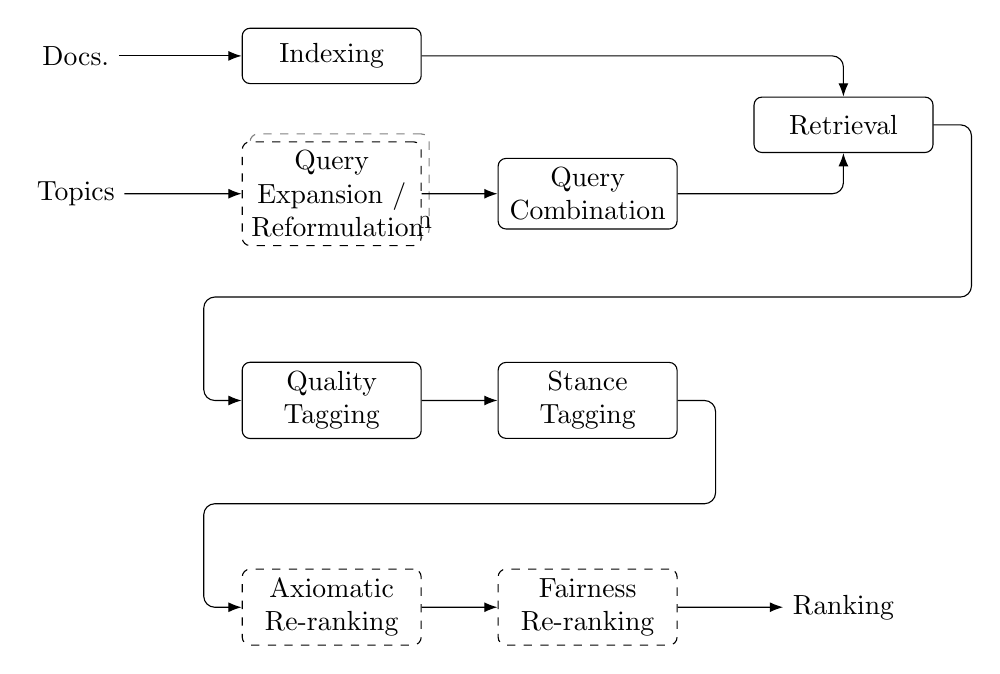
\begin{tikzpicture}[
        xscale=3.25,
        yscale=-1.75,
        block/.style={
            rectangle,
            draw,
            fill=white,
            text centered,
            rounded corners=1mm,
            text width=5.8em,
            minimum height=2em
        },
        line/.style={
            draw,
            -Latex,
            rounded corners
        },
        ]

        \node (documents) at (0,0) {Docs.};
        \node [block] (index) at (1,0) {Indexing};
        \node (topics) at (0,1) {Topics};
        \node [block,dashed,draw opacity=0.5,xshift=1mm,yshift=1mm] at (1,1) {Query Expansion / \\ Reformulation};
        \node [block,dashed] (query-expansion-reformulation) at (1,1) {Query Expansion / \\ Reformulation};
        \node [block] (query-combining) at (2,1) {Query Combination};
        \node [block] (retrieval) at (3,0.5) {Retrieval};
        \node [block] (quality-tagging) at (1,2.5) {Quality Tagging};
        \node [block] (stance-tagging) at (2,2.5) {Stance Tagging};
        \node [block,dashed] (axiomatic-reranking) at (1,4) {Axiomatic Re-ranking};
        \node [block,dashed] (fairness-reranking) at (2,4) {Fairness Re-ranking};
        \node (ranking) at (3,4) {Ranking};
ranking
        \path [line] (documents) -- (index);
        \path [line] (topics) -- (query-expansion-reformulation);
        \path [line] (query-expansion-reformulation) -- (query-combining);
        \path [line] (index) -| (retrieval);
        \path [line] (query-combining) -| (retrieval);
        \path [line] (retrieval) -| (3.5,1.5) |- (2,1.75) -| (0.5,2) |- (quality-tagging);
        \path [line] (quality-tagging) -- (stance-tagging);
        \path [line] (stance-tagging) -| (2.5,3) |- (2,3.25) -| (0.5,3.5) |- (axiomatic-reranking);
        \path [line] (axiomatic-reranking) -- (fairness-reranking);
        \path [line] (fairness-reranking) -- (ranking);
    \end{tikzpicture}\\[0.75em]
	\caption{Architecture overview for the retrieval pipeline used to produce our runs. Dashed boxes indicate optional steps, that are not used in all runs.}
    \label{figure-pipeline}
\end{figure}


We design the architecture of our argumentative retrieval system as a pipeline of multiple steps that subsequently (re-)rank, annotate, or modify the documents or queries given as inputs. This pipeline is shown in Figure~\ref{figure-pipeline}.
We identify four core steps as most important to our approach:
\Ni query expansion, reformulation, and combination,
\Nii first-stage retrieval,
\Niii argument quality and stance tagging,
and \Niv axiomatic reranking and fairness reranking.

Additionally, we add an evaluation component that is not shown in Figure~\ref{figure-pipeline} because it is not needed to retrieve results from our system.
With this evaluation component we can evaluate our system on topics of previous editions~(i.e.,~2021 and~2020) of the Touché Lab on Argument Retrieval~(c.f.~Section~\ref{transfer-relevance-judgements}).

\subsection{Query Expansion, Reformulation, and Combination}
\label{reformulation}

In order to increase recall of our first-stage ranker and to include results for very similar yet differently named objects, we first expand and reformulate the original search query.
Our approaches use two different strategies: \Ni we replace the comparative objects with their synonyms and \Nii we generate additional, new queries using the additional description and narrative information provided by the shared task organizers.
Expanding the original query with synonyms of comparative objects is motivated by the fact that documents often contain more specific comparisons~(e.g., Ubuntu vs Windows) instead of more broad comparisons~(e.g., Linux vs Windows).
Yet, specific examples of a more general class of objects are useful to answer comparative questions about their object class.
We might therefore find relevant documents that would otherwise not match any original query term.
It is however important to note that increasing recall can result in an decrease in precision which is undesirable in the precision-oriented setting of the shared task.
However, we later apply re-ranking steps that improve precision by moving irrelevent documents further down the ranking~(c.f.~Section~\ref{reranking}).

\paragraph{Query Expansion with Synonyms}

We use two different strategies to find synonyms: \Ni word embeddings and \Nii a zero-shot language model.
In our first strategy, we use fastText word embeddings~\cite{BojanowskiGJM2017} to find words with the highest cosine similarity to the given comparative objects in the embedding space.
We manually examine synonyms from fastText embeddings using different domains~(i.e., Wikipedia and Twitter) and find that fastText embeddings trained on the Twitter corpus result in the best synonyms.

Our second strategy to obtain synonyms is based on the T0++~zero-shot language model~\cite{SanhWRBSACSLRDBXTSSKCNDCJWMSYPBWNRSSFFTBGBWR2021}.
We ask the model to generate an answer to the following task: \query{What are synonyms of the word~<token>?} where \query{<token>}~is one of the two comparative objects.
From the text returned by the language model, we then parse synonyms by splitting at commas and remove duplicate synonyms.
With the synonyms returned by either strategy, we replace the comparative objects to form new queries. All alternative queries and the original query are then combined.

\paragraph{Query Reformulation with Topic Context}

\begin{table}
    \caption{Original queries provided by \citet{BondarenkoFKSGBPBSWPH2022} and newly generated queries by T0++~\cite{SanhWRBSACSLRDBXTSSKCNDCJWMSYPBWNRSSFFTBGBWR2021} using the topic's description~(D) or narrative~(N).}
    \label{table-generated-queries}
    \begin{tabularx}{\linewidth}{c >{\hsize=.7\hsize\linewidth=\hsize}X c >{\hsize=1.3\hsize\linewidth=\hsize}X}
        \toprule
        \textbf{Topic} & \textbf{Original Query} & \textbf{Field} & \textbf{Generated Query} \\
        \midrule
        \multirow{2}{*}{12} & \multirow{2}{\linewidth}{Train or plane? Which is the better choice?} & D & Travel \\
        & & N & What are the benefits of trains over planes for intercontinental travel? \\
        \multirow{2}{*}{53} & \multirow{2}{\linewidth}{Should I buy steel or ceramic knives?} & D & Why should I choose ceramic knives over steel knives? \\
        & & N & What are the pros and cons of ceramic knives? \\
        \multirow{2}{*}{88} & \multirow{2}{\linewidth}{Should I major in philosophy or psychology?} & D & What is the difference between philosophy and psychology? \\
        & & N & What are the benefits of a major in English or history? \\
        \multirow{2}{*}{95} & \multirow{2}{\linewidth}{Which is more environmentally friendly, a hybrid or a diesel?} & D & What are the most environmentally friendly cars? \\
        & & N & What is more environmentally friendly, a diesel or a hybrid car? \\
        \bottomrule
    \end{tabularx}
\end{table}


We complement the queries expanded by replacing synonyms with newly generated queries that incorporate the contextual information provided in description narrative fields from the shared task's topics.
The description contains important details about the actual information need and the narrative clearly defines which passages are relevant for the query.
We use this valuable information about which passages to retrieve by generating new queries with the T0++ language model~\cite{SanhWRBSACSLRDBXTSSKCNDCJWMSYPBWNRSSFFTBGBWR2021} and providing it with a topic's description or narrative.

We challenge the T0++ model with the following task: \query{<text>.~Extract a natural search query from this description.} where \query{<text>}~is either the topic's narrative or description.
The string returned by the language model is then used as is as the new query for the topic and combined with the previous queries.
In Table~\ref{table-generated-queries}, we show examples of generated queries.
Albeit some of the generated queries~(e.g., topic~53) are just reformulations of the original query, the T0++ language model gernerates some interesting new queries for other topics~(e.g., topic~12).

\paragraph{Disjunctive Query Combination}
After the query expansion and query reformulation steps, we need to combine all computed queries and the original query.
We decide to combine all queries in a single query in a logical disjunction, that is by using Pyserini's OR operator.
Two reasons influence this decision:
Firstly, retrieving results for just one query is conceptually easier as we don't neet to interleave multiple result sets after the retrieval step.
Interleaving is not trivial and it is often challenging to find an interleaving strategy without many caveats.
Secondly, the logical disjunction increases the system's recall and decrease the chance of empty result sets in the cse that a term is not present in the corpus.
Although, the query reformulation, expansion and combination steps are optional, meaning that we use these steps only in some runs. In most of our submitted runs, we just use the original query, because the increase in recall might result in a decreasequery in precision that is hard to offset in subsequent re-ranking steps.

\subsection{Passages Retrieval}\label{retrieval}

To retrieve passages from the set of passages extracted from ClueWeb~12 by the task organizers, we first build an inverted index using the Pyserini framework~\cite{LinMLYPN2021}.
Pyserini allows for experimenting with multiple steps of a retrieval system including indexing and simple retrieval models like Okapi~BM25 or the query likelihood model.
In the index, we store index term positions, passage vectors, and raw passage contents.
Index terms are stemmed using the Porter stemmer~\cite{Porter1980} and stop words are removed as per the default Pyserini stopword list~\cite{LinMLYPN2021}.
We then retrieve passages for the previously combined query~(c.f. Section~\ref{reformulation}) using the query likelihood model with Dirichlet smoothing~(\( \mu = 1000 \)) in Pyserini.
From this first-stage ranker, we retrieve 100~candidate passages for each query.

\subsection{Argument Quality and Stance Tagging}

After retrieving candidate passages, we tag the argumentative quality and argument stance.
Both quality and stance are required for later steps in our retrieval pipeline to re-rank the passages~(c.f. Section~\ref{reranking}).
Also, the task organizers ask the participants to optionally return a stance for each retrieved document as a sub-task in the Touché Lab on Argument Retrieval.
In order to tag each passage's quality and stance we first split each retrieved passage into sentences using the NLTK library~\cite{BirdLK2009}.
Then each sentence is treated as one potential argument and tagged with its argumentative quality and stance.
To find the quality score and stance for the whole passage, we average the quality or stance scores respectively of all sentences in the passage.

\paragraph{Argument Quality Tagging}
\begin{table}
    \caption{Argument quaity label mapping for textual labels returned by the T0++~language model~\cite{SanhWRBSACSLRDBXTSSKCNDCJWMSYPBWNRSSFFTBGBWR2021}.}
    \label{table-quality-mapping}
    \begin{tabular}{lc}
        \toprule
        \textbf{Text Label} & \textbf{Value} \\
        \midrule
        \query{very good} & 1.00 \\
        \query{good} & 0.75 \\
        \query{bad} & 0.25 \\
        \query{very bad} & 0.00 \\
        other & 0.50 \\
        \bottomrule
    \end{tabular}
\end{table}


We implement two different methods for quality tagging:
Our first method is based on the IBM Debater API~\footnote{\url{https://early-access-program.debater.res.ibm.com}}~\cite{ToledoGCFVLJAS2019}.
Here we send each sentence from one passage and the original query as the topic to the IBM Debater API for argument quality assessment. of Passages
The API then determines how good the quality of each argument with regards to the topic is with a \Bert-based regression classifier model trained on the IBM-ArgQ-6.3kArgs dataset. The model and therefore the API then returns a quality score ranging from 0 to 1 where a classified score of~0 means very poor argument quality and a score of~1 means very good argument quality~\cite{ToledoGCFVLJAS2019}.

As a second method to obtain the argument quality we again use the T0++ language model~\cite{SanhWRBSACSLRDBXTSSKCNDCJWMSYPBWNRSSFFTBGBWR2021}.
We ask the T0++ model to generate a text the following task: \query{<sentence>.~How would you rate the readability and consistency in this sentence? very good, good, bad, very bad} where \query{<sentence>}~is one sentence of a passage.
This results in an output of either \query{very good}, \query{good}, \query{bad}, or \query{very bad} depending on how the pretrained T0++ model interprets the sentence's argument quality.
We then map this textual output labels to numeric values as per the mapping shown in Table~\ref{table-quality-mapping}.

\paragraph{Argument Stance Tagging}
\begin{table}
    \caption{Argument stance label mapping for textual labels returned by the T0++~language model~\cite{SanhWRBSACSLRDBXTSSKCNDCJWMSYPBWNRSSFFTBGBWR2021} for positive~(Pro) and negative~(Con) stance towards a single comparative object.}
    \label{table-stance-mapping}
    \begin{tabular}{llc}
        \toprule
        \multicolumn{2}{c}{\textbf{Text Label}} & \textbf{Value} \\
        Pro & Con & \\
        \midrule
        \query{yes} / \query{pro} & \query{yes} / \query{con} & \phantom{-}0 \\
        \query{yes} / \query{pro} & \query{no} & +1 \\
        \query{no} & \query{yes} / \query{con} & -1 \\
        \query{no} & \query{no} & \phantom{-}0 \\
        other & other & \phantom{-}0 \\
        \bottomrule
    \end{tabular}
\end{table}


Stance detection for each sentence uses the same conceptual approaches but with different inputs and outputs.
Since both the IBM Debater API~\cite{BarHaimBDSS2017} and our T0++ approach~\cite{SanhWRBSACSLRDBXTSSKCNDCJWMSYPBWNRSSFFTBGBWR2021} are only capable of calculating a single-target stance~(i.e., for one of the two comparative objects), we combine the two single-target stances into a multi-target stance by taking the difference between the stance towards the first comparative object and the stance towards the second comparative object.
We also experimented with different thresholds for the minimal difference between the single-target stances but found no improvements in the combined, multi-target stance when manually examining some classified examples.

For scoring the single-target argument stance for a sentence with the IBM Debater API, we again send the sentence and a claim built using one of the comparative objects to the IBM Debater API.
The classifier by \citet{BarHaimBDSS2017} computes an argument's likelihood of being pro, con, or neutral with respect to the claim~(i.e., the comparative object in our pipeline) by first classifying sentiments and then detecting contrasts in the topic and argument claim targets.
The API then returns a score from from~-1 to~+1 where -1~means the argument is against the comparative object and +1~means that the argument is in favor of the comparative object.
By classifying different claims for each object~(i.e., \query{<object>~is good} and \query{<object>~is the best}), we get an averaged single-target stance for each comparative object.

For the second method using the T0++~language model~\cite{SanhWRBSACSLRDBXTSSKCNDCJWMSYPBWNRSSFFTBGBWR2021} we first experiment with directly asking the model to generate~\query{pro}, \query{con}~or~\query{neutral} classification labels for a comparative object.
However, we found that the T0++ model would not be able to reliably distinguish between a positive and negative stance towards the comparative object.
Therefore we instead reformulate the task in two simple questions, one to determine whether the sentence has a positive stance towards the comparative object and one to determine whether it has a negative stance: \query{<sentence> Is this sentence pro <object>? yes or no} and \query{<sentence> Is this sentence against <object>? yes or no} where \query{<sentence>}~is one sentence of the passage and \query{<object>}~is one of the comparative objects.
This results in two answers~(\query{yes} or~\query{no}) for the positive and negative stance respectively. We combine the two textual answers as shown in Table~\ref{table-stance-mapping} and then combine the single-target stances into a multi-target stance as described above.

\subsection{Axiomatic Reranker}
\label{reranking}

\begin{table}
    \caption{Axioms used in our pipeline. Axioms without citations are our own work.}
    \label{table-axioms}
    \begin{tabular}{ll}
        \toprule
        \textbf{Name} & \textbf{Description} \\
        \midrule
        ArgUC~\cite{BondarenkoHVSPB2018} & Prefer more argumentative units. \\
        QTArg~\cite{BondarenkoHVSPB2018} & Prefer more query terms in argumentative units. \\
        QTPArg~\cite{BondarenkoHVSPB2018} & Prefer earlier query terms in argumentative units. \\
        CompArg & Prefer more comparative objects in argumentative units. \\
        CompPArg & Prefer earlier comparative objects in argumentative units. \\
        aSLDoc~\cite{BondarenkoFKHVS2019} & Prefer passages with 12--20 words per sentence. \\
        ArgQ & Prefer higher argument quality. \\ 
        \bottomrule
    \end{tabular}
\end{table}


At the end of our pipeline is the axiomatic reranker which will rerank the retrieved passages from our retrieval step (c.f. Section~\ref{retrieval}).
We use a reranker because in our first pipeline step we increased the recall by using different queries instead of just the original one.
But a good retrieval result set will be precision focused.
The reranker will help us to rearrange the passage in a manner so that the best passages will be at the top of the resulting ranking and therefore we will optimize for measurements that lay their focus on the top results rather than the whole set.
To accomplish this task we will compute preferences between passages via axioms.
Axioms are rules which will vote for or against the original ranking.
By computing axioms between pairs of passages, we can observe which passage should be above or below another passage.
For re-ranking, we use the \iraxioms framework\footnote{\url{https://github.com/webis-de/ir_axioms/}} with the \KwikSort algorithm~\cite{HagenVGS2016}.
In Table \ref{table-axioms} we list the axioms used in our pipeline.

Additional to this reranker which only relies on axioms we also implemented a fairness reranker whose purpose is to produce fair rankings. Fair here means that pro and con arguments appear balanced while preferring subjective arguments over neutral arguments. For this reranking approach, we implemented two different strategies. The first strategy is called alternating stance. Here we have three lists one with only pro arguments regarding comparative object 1, one with only pro arguments regarding comparative object 2, and one with neutral arguments. We then alternately select from the first two lists. If one or both lists are empty we fall back to the neutral list. The second strategy is called balanced top-k stance. Here we count the passages pro the first comparative object and pro the second comparative object in our top-k ranking. If the difference between the two numbers is greater than 1 we move the last pro first comparative object passage from the top-k ranking after the first pro-second comparative object passage after the top-\(k\) ranking.

\subsection{Submitted Runs}

\todo{Shortly describe the 5 submitted runs.}
\section{Evaluation} \label{evaluation}
    The approach has been successfully deployed on the evaluation platform Tira\footnote{https://www.tira.io/}. Our approach can be found under the name XXXX. Tira automatically evaluates the submitted approaches of the participants of the shared task and reports the NDCG@5. The organizers use this site to ensure a reproducible leaderboard. We will now have a closer look at the performance of our approach by looking at the first 5 results of three chosen topics for two different runs. The two runs we are looking at are (1) without query reformulation/expansion and axiomatic reranking and (2) with query reformulation/expansion and axiomatic reranking.
    \subsection{Topic 1}
        The first query we will have a look at will be: \textit{Which is better, a laptop or a desktop?} According to the narrative field provided by the organizers' passages that contain major similarities and dissimilarities of laptops and desktops are relevant. Also relevant are passages which contain advantages and disadvantages of specific usage scenarios.
        \subsubsection*{Run 1}
            The first returned passage contains arguments for laptops and also for desktops while being subjective and non-biased. Our second and fifth results are product descriptions of laptops and do not deliver arguments for or against laptops/desktops. The third returned passage shows us results for laptops on a website where we can buy laptops. Our fourth result gives us 5 arguments why laptops are better. So manually we would  change the ranking as follows: 1-4-2-5-3
        \subsubsection*{Run 2}
            Our second run retrieves passages on its first three places which are about different laptops. These websites give a detailed overview of the laptop they are talking about but no argument for or against laptops/desktops is given. On our fourth place, we have a review for a network switch. The fifth place is a selling website for electronic products. We must admit that the first five results are not relevant and do not provide argumentative support to the user. The passage which was our first place in our first run is now in place 34. An explanation might be that using synonyms, in this case, lead to inaccurate search queries which did not capture the user's information need.
    \subsection{Topic 2}
        The next question we will have a look at is: \textit{Is OpenGL better than Direct3D in terms of portability to different platforms?} Relevant passages should contain information about the portability of OpenGL/Direct3D across different operation systems. Not relevant are ads or tutorials for OpenGL/Direct3D.
        \subsubsection*{Run 1}
            The first result talks about 3D-rendering in the Opera browser and does not provide any arguments. The second done is a gaming-related blog post again no arguments are given. The third and fourth results are the same page (but different ClueWeb-ID) and talk about a gaming developer who converted his game from OpenGL to Direct3D. He talks about his problems and gives tips on which pattern to avoid while developing a 3D game. In our last passage, we can get the information that Direct3D is now supported in Linux. The only passages which are kind of relevant are the third and fourth. All other of the first five passages are not relevant. 
        \subsubsection*{Run 2}
            The returned results are the same passages returned by run 1 but in a different order. The first two passages are the ones that talk about the game developer and his problems converting from OpenGL to Direct3D. Then we will get the passage which is about the support of Direct3D in Linux. In fourth place we have the passage talking about the 3D-rendering in Opera and the last result is the gaming-related blog. So the ranking has slightly improved since the most relevant passages are now in place 1 and 2 while other less relevant passages are now further behind in the ranking.
    \subsection{Topic 3}
        Our last topic will be: \textit{Which technology performs better: Apple's or Google's?} Relevant passages should compare both companies in terms of service and their products. Relevant passages can focus on one company. Not relevant passages are about genric information about the companies.
        \subsubsection*{Run 1}
            The first passage returned is a news site about technology and talks about various topics from this domain but no arguments are given. The second passage talks about the new Google TV while AppleTV has been already released. In the third place, there is a passage that talks about how Apple and Google both signed a privacy accord. The fourth result is about Facebook buying Instagram. The last result is about Google being caught violating users' privacy while Apple has been already caught violating users' privacy. So we have some relevant passages here. We would rank the passages as follows: 3-5-2-4-1. So the top-5 ranking is not very good. 
        \subsubsection*{Run 2}
            The first passage is a news site about Apple products and provides some insight into these products. The second passage provides information about selling numbers and stock prices. So this site is not relevant according to the narrative provided by the organizers. The next passage is a news article about how Google and Motorola have to hand over Android information to Apple. So no arguments are provided in this passage. The fourth result is about how Apple could only have success because of Google.  The last passage talks about five reasons iPhone vs Android is not Mac vs Windows. So we can see that different passages have been retrieved for run 1 and run 2. For run 2 we would rank the passages as follows: 1-4-5-3-2.
\section{Conclusion}

We have seen an approach to tackle the task of answering comparative questions and detecting the stance of the returned passages regarding the comparative objects.
Our approach combines query reformulation/expansion techniques with axiomatic reranking and shows two principle ways of determining the argument quality and stance.
Our work expands previous work from earlier years of the shared task by using different techniques to expand the original queries and also incorporates the information from the description and narrative field.
We also use axiomatic reranking in contrast to reranking based solely on weighting scores.

We have seen in Section~\ref{evaluation} that query expansion/reformulation and the additional information from the narrative and description field can provide a better search result.
But it is also possible that the result gets slightly worse in comparison to not using query expansion/reformulation at all.
This is because with these techniques we will alter the search terms used and some synonyms could lead to passages that do not comply with the user's information need.
The axiomatic reranking proves to be robust and reliable but sometimes it can not compensate for the errors from the query expansion/reformulation and passages which were relevant will be further down in the ranking.

Difficulties arise for our stance classification since we solely rely on external APIs which only provide a single-target stance.
Firstly, computing the multi-target stance from a single-target stance proved to be challenging.
Second, our approach can not decide between no argument present and neutral stance which is a big caveat.
The performance of our classification could be improved by using \Bert models or other machine learning-based approaches which can predict a multi-target stance.
An interesting question arose during our research:
Is it possible to only use the language model T0 to develop an information retrieval pipeline?
We look forward to evaluate this question in more detail with relevance judgements provided by the shared task organizers~\cite{BondarenkoFKSGBPBSWPH2022}.

There are many different challenging problems to solve to create an information retrieval pipeline to answer comparative questions.
Our approach proposed several possibilities for how to solve them each with its limitations and caveats.


\begin{acknowledgments}
  We thank Huggingface for providing us access to their hosted inference API\footnote{\url{https://api-inference.huggingface.co}} to generate texts with the T0++~model, which would otherwise not have been possible due to hardware constraints. 
  We are also grateful to the Webis group for hosting the TARGER API and to IBM Research for early access to their Debater APIs.
\end{acknowledgments}

\bibliography{literature}

\end{document}
